\documentclass[utf8x]{beamer}

% This file is a solution template for:

% - Talk at a conference/colloquium.
% - Talk length is about 20min.
% - Style is ornate.

\mode<presentation>
{
  \usetheme{Warsaw}
  % or ...

  %\setbeamercovered{transparent}
  % or whatever (possibly just delete it)
}


\usepackage[english]{babel}
\usepackage{listings}
\usepackage{ulem}
\usepackage{color}
\usepackage{alltt}

\usepackage[utf8x]{inputenc}


\newcommand\redsout[1]{{\color{red}\sout{\hbox{\color{black}{#1}}}}}

% or whatever

% Or whatever. Note that the encoding and the font should match. If T1
% does not look nice, try deleting the line with the fontenc.


\title{Allocation Removal by Partial Evaluation in a Tracing JIT}

\author[Carl Friedrich Bolz et. al.]{\emph{Carl Friedrich Bolz}\inst{1} \and Antonio Cuni\inst{1} \and Maciej Fijałkowski\inst{2} \and Michael Leuschel\inst{1} \and Samuele Pedroni\inst{3} \and Armin Rigo\inst{1}}
% - Give the names in the same order as the appear in the paper.
% - Use the \inst{?} command only if the authors have different
%   affiliation.

\institute[Heinrich-Heine-Universität Düsseldorf]
{$^1$Heinrich-Heine-Universität Düsseldorf, STUPS Group, Germany \and

 $^2$merlinux GmbH, Hildesheim, Germany \and

 $^3$Open End, Göteborg, Sweden \and
}

\date{2011 Workshop on Partial Evaluation and Program Manipulation, January 24, 2011}
% - Either use conference name or its abbreviation.
% - Not really informative to the audience, more for people (including
%   yourself) who are reading the slides online


% If you have a file called "university-logo-filename.xxx", where xxx
% is a graphic format that can be processed by latex or pdflatex,
% resp., then you can add a logo as follows:




% Delete this, if you do not want the table of contents to pop up at
% the beginning of each subsection:
%\AtBeginSubsection[]
%{
%  \begin{frame}<beamer>
%    \frametitle{Outline}
%    \tableofcontents[currentsection,currentsubsection]
%  \end{frame}
%}


% If you wish to uncover everything in a step-wise fashion, uncomment
% the following command: 

%\beamerdefaultoverlayspecification{<+->}


\begin{document}

\begin{frame}
  \titlepage
\end{frame}

% XXX todos:
% note that two fields is a simplification
% have a diagram for the example trace
% lifting can never produce new operations
% have some sort of overview or position indicator for the many graphical slides, too easy to get lost
% more details about benchmarks, diagram?


% Structuring a talk is a difficult task and the following structure
% may not be suitable. Here are some rules that apply for this
% solution: 

% - Exactly two or three sections (other than the summary).
% - At *most* three subsections per section.
% - Talk about 30s to 2min per frame. So there should be between about
%   15 and 30 frames, all told.

% - A conference audience is likely to know very little of what you
%   are going to talk about. So *simplify*!
% - In a 20min talk, getting the main ideas across is hard
%   enough. Leave out details, even if it means being less precise than
%   you think necessary.
% - If you omit details that are vital to the proof/implementation,
%   just say so once. Everybody will be happy with that.

\begin{frame}
  \frametitle{Dynamic Languages are Slow}
  \begin{itemize}
      \item Interpretation overhead
      \item Type dispatching
      \item Boxing of primitive types
      \pause
      \begin{itemize}
          \item A lot of allocation of short-lived objects
      \end{itemize}
  \end{itemize}
\end{frame}

\begin{frame}
  \frametitle{Dynamic Languages are Slow: Example}
  \texttt{x = a + b; y = x + c}

  evaluated in an interpreter:
  \pause
  \begin{enumerate}
      \item What's the type of a? \texttt{Integer}
      \item What's the type of b? \texttt{Integer}
  \pause
      \item unbox a
      \item unbox b
      \item compute the sum
  \pause
      \item box the result as an \texttt{Integer}
      \item store into x
  \pause
      \item What's the type of x? \texttt{Integer}
      \item What's the type of c? \texttt{Integer}
  \pause
      \item unbox x
      \item unbox c
      \item compute the sum
  \pause
      \item box the result as an \texttt{Integer}
      \item store into y
  \end{enumerate}
\end{frame}

\begin{frame}
  \frametitle{What to do?}
  \begin{itemize}
      \item Use a JIT compiler
      \item \textbf{Add an optimization that can deal with heap operations}
      \pause
      \item optimize short-lived objects
      \item remove some of the redundant type checks
  \end{itemize}
\end{frame}

\begin{frame}
  \frametitle{Overview}
  \tableofcontents
  % You might wish to add the option [pausesections]
\end{frame}

\section{Experimental Context}

\begin{frame}
  \frametitle{Our Experimental Context is the PyPy Project}
  A general environment for implementing dynamic languages
  \pause
  \begin{block}{Approach}
      \begin{itemize}
          \item write an interpreter for the language in RPython
          \item compilable to an efficient C-based VM
          \pause
          \item (RPython is a restricted subset of Python)
      \end{itemize}
  \end{block}
\end{frame}

\begin{frame}
  \frametitle{PyPy Uses a Novel Tracing JIT}
  the feature that makes PyPy interesting:
  \begin{itemize}
      \item a meta-JIT, applicable to many languages
      \item needs a few source-code hints (or user annotations) in the interpreter
      \item JIT is a tracing JIT compiler
  \end{itemize}
\end{frame}

\begin{frame}
  \frametitle{Tracing JITs Compile by Observing an Interpreter}
  \begin{itemize}
      \item VM contains both an interpreter and the tracing JIT compiler
      \item JIT works by observing and logging what the interpreter does
      \begin{itemize}
          \item for interesting, commonly executed code paths
          \item produces a linear list of operations (trace)
      \end{itemize}
      \item trace is optimized and then turned into machine code
  \end{itemize}
\end{frame}

\begin{frame}
  \frametitle{The Advantages of Tracing JITs}
  \begin{itemize}
      \item Traces are interesting linear pieces of code
      \item most of the time correspond to loops
      \item everything called in the trace is inlined
      \item can perform good optimizations on the trace
      \item rarer paths run by the interpreter
  \end{itemize}
\end{frame}

\begin{frame}[containsverbatim]
  \frametitle{Example Trace}
  Trace of \texttt{x = a + b; y = x + c}:
\begin{verbatim}
guard_class(a, Integer)
guard_class(b, Integer)
i1 = get(a, intval)
i2 = get(b, intval)
i3 = int_add(i1, i2)
x = new(Integer)
set(x, intval, i3)
\end{verbatim}
\pause
\begin{verbatim}
guard_class(x, Integer)
guard_class(c, Integer)
i4 = get(x, intval)
i5 = get(c, intval)
i6 = int_add(i4, i5)
y = new(Integer)
set(y, intval, i6)
\end{verbatim}
\end{frame}

\begin{frame}[containsverbatim]
  \frametitle{Example Trace}
  Trace of \texttt{x = a + b; y = x + c}:
\begin{verbatim}
guard_class(a, Integer)
guard_class(b, Integer)
i1 = get(a, intval)
i2 = get(b, intval)
i3 = int_add(i1, i2)
x = new(Integer)
set(x, intval, i3)
\end{verbatim}
\begin{verbatim}
guard_class(x, Integer)
guard_class(c, Integer)
i4 = get(x, intval)
i5 = get(c, intval)
i6 = int_add(i4, i5)
y = new(Integer)
set(y, intval, i6)
return(y)
\end{verbatim}
\end{frame}

\begin{frame}[containsverbatim]
  \frametitle{Optimized Example Trace}
  Trace of \texttt{x = a + b; y = x + c}:
\begin{alltt}
guard_class(a, Integer)
guard_class(b, Integer)
i1 = get(a, intval)
i2 = get(b, intval)
i3 = int_add(i1, i2)
\redsout{x = new(Integer)}
\redsout{set(x, intval, i3)}
\end{alltt}
\begin{alltt}
\redsout{guard_class(x, Integer)}
guard_class(c, Integer)
\redsout{i4 = get(x, intval)}
i5 = get(c, intval)
i6 = int_add(\emph{i3}, i5)
y = new(Integer)
set(y, intval, i6)
return(y)
\end{alltt}
\end{frame}

\section{Proposed Optimization}

\begin{frame}
  \frametitle{Contribution of our Paper}
  \begin{itemize}
      \item a simple, efficient and effective optimization of heap operations in a trace
      \item using online partial evaluation
      \item fully implemented and in use in large-scale interpreters
  \end{itemize}
  \pause
  \begin{block}{Ingredients}
      \begin{itemize}
          \item a slightly simplified model for objects on the heap
          \item operational semantics of trace operations that manipulate the heap
          \item optimization rules for those operations, following the operational semantics
      \end{itemize}
  \end{block}
\end{frame}



\begin{frame}
  \frametitle{Heap Model}
  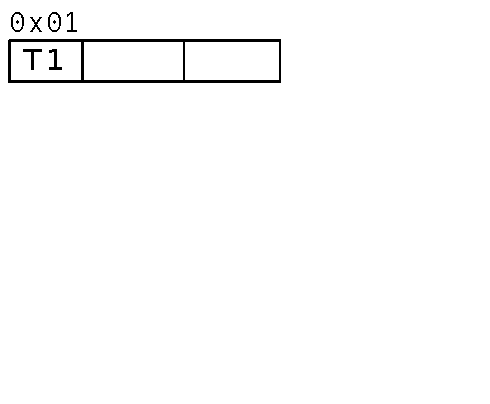
\includegraphics[scale=0.9]{figures/heap01}
\end{frame}

\begin{frame}
  \frametitle{Heap Model}
  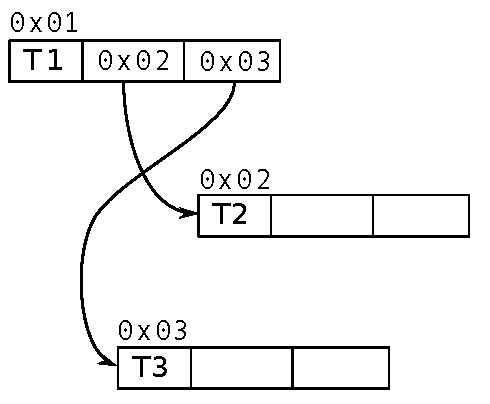
\includegraphics[scale=0.9]{figures/heap02}
\end{frame}

\begin{frame}
  \frametitle{Heap Model}
  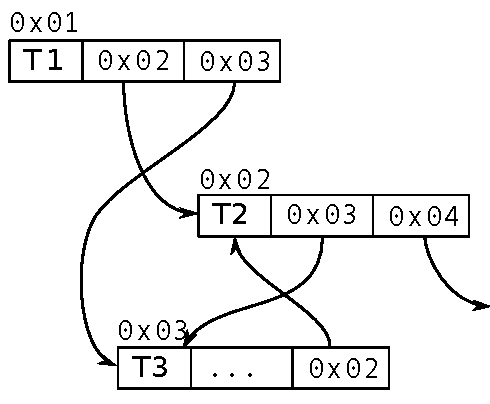
\includegraphics[scale=0.9]{figures/heap03}
\end{frame}

\begin{frame}
  \frametitle{Operations Manipulating Heap Objects}
  \begin{itemize}
      \item \texttt{v = new(T)} makes a new object
      \item \texttt{u = get(w, F)} reads a field out of an object
      \item \texttt{set(v, F, w)} writes a field of an object
      \item \texttt{guard(v, T)} checks the type of an object
  \end{itemize}
\end{frame}

\begin{frame}[plain]
  \frametitle{Operations: New}
%  \begin{columns}[c]
%  \begin{column}{10cm}
    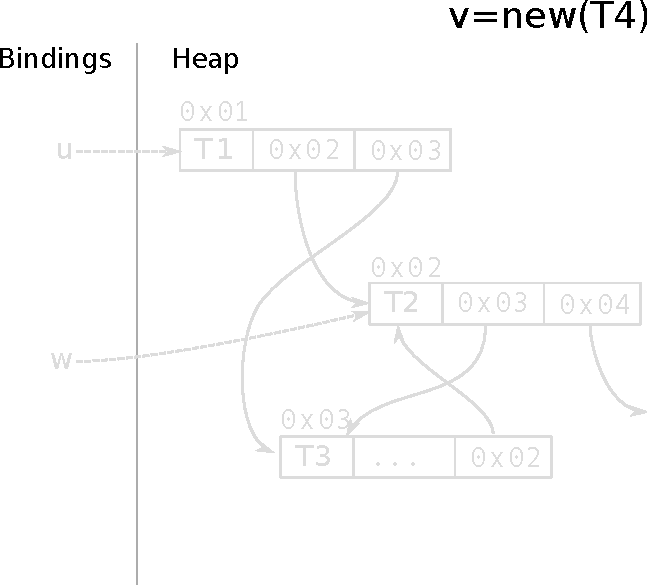
\includegraphics[scale=0.8]{figures/new01}
%  \end{column}
%  \begin{column}{2cm}
%  {\tiny 
%  \begin{itemize}
%    \item new
%    \item get
%    \item set
%    \item guard
%  \end{itemize}
%  }
%  \end{column}
%  \end{columns}
\end{frame}

\begin{frame}[plain]
  \frametitle{Operations: New}
  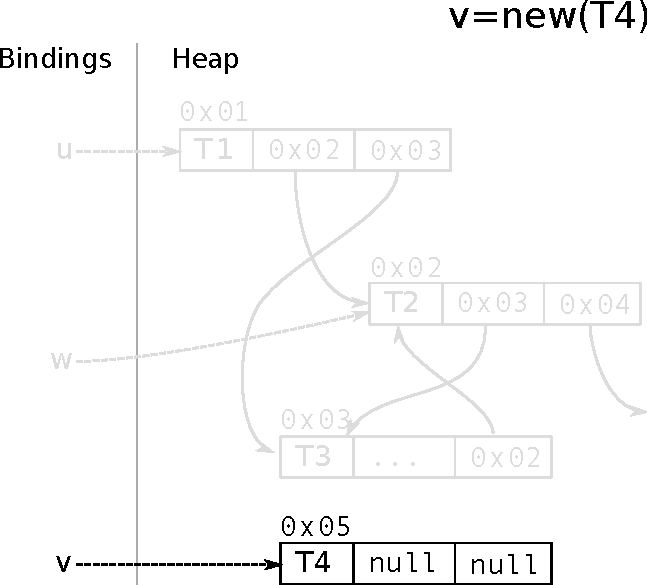
\includegraphics[scale=0.8]{figures/new02}
\end{frame}

\begin{frame}[plain]
  \frametitle{Operations: Get}
  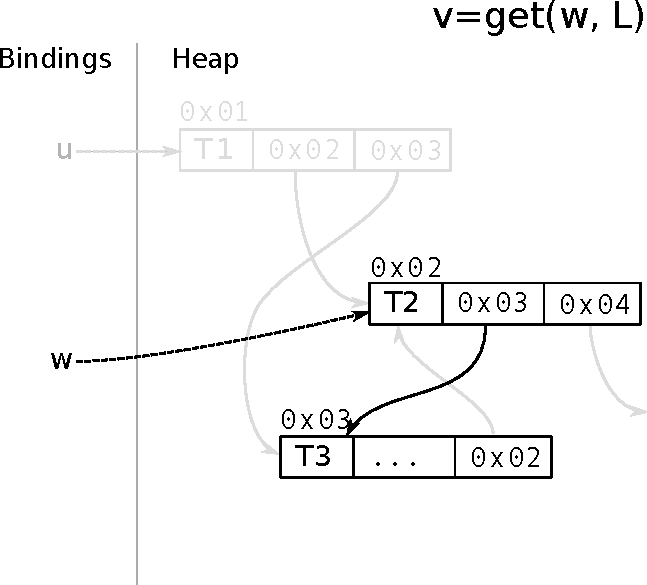
\includegraphics[scale=0.8]{figures/get01}
\end{frame}

\begin{frame}[plain]
  \frametitle{Operations: Get}
  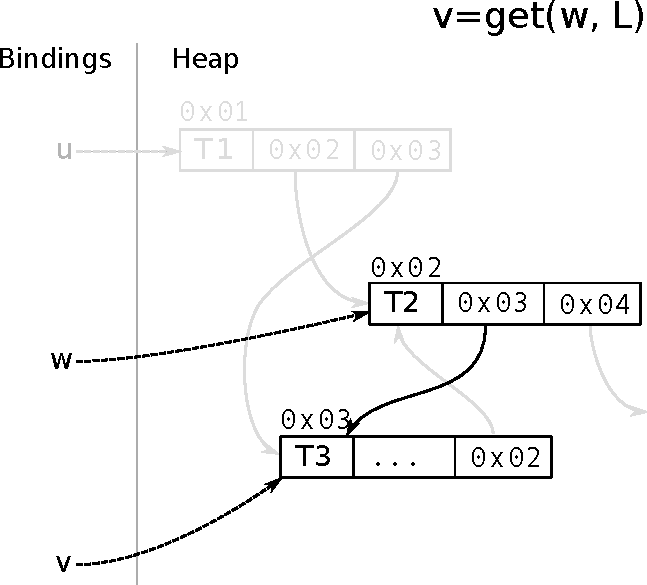
\includegraphics[scale=0.8]{figures/get02}
\end{frame}

\begin{frame}[plain]
  \frametitle{Operations: Set}
  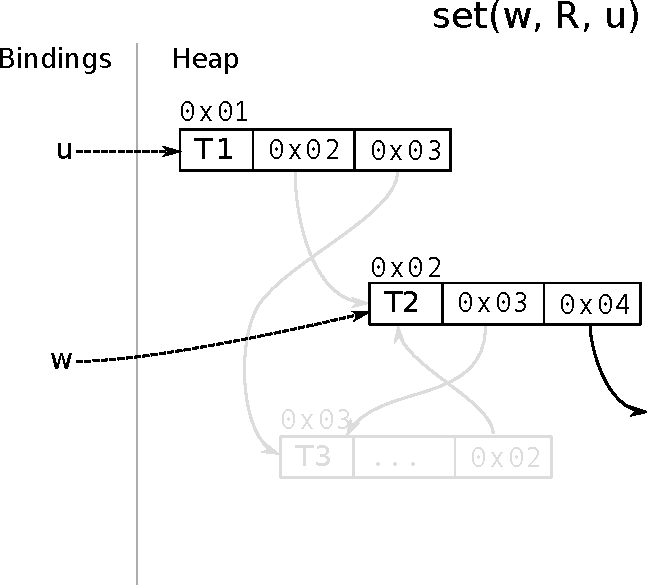
\includegraphics[scale=0.8]{figures/set01}
\end{frame}

\begin{frame}[plain]
  \frametitle{Operations: Set}
  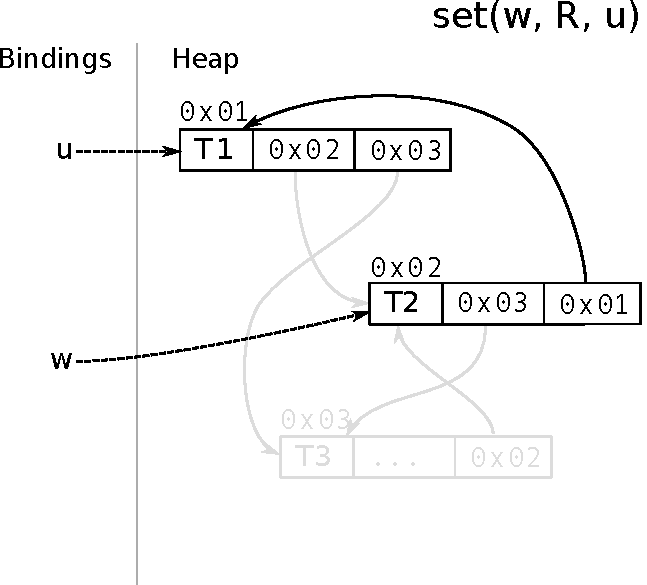
\includegraphics[scale=0.8]{figures/set02}
\end{frame}

\begin{frame}[plain]
  \frametitle{Operations: Guard}
  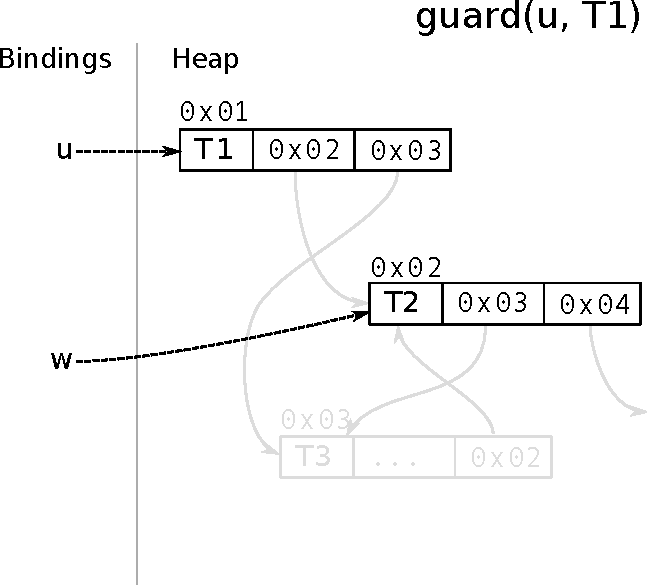
\includegraphics[scale=0.8]{figures/guard01}
\end{frame}

\begin{frame}[plain]
  \frametitle{Operations: Guard}
  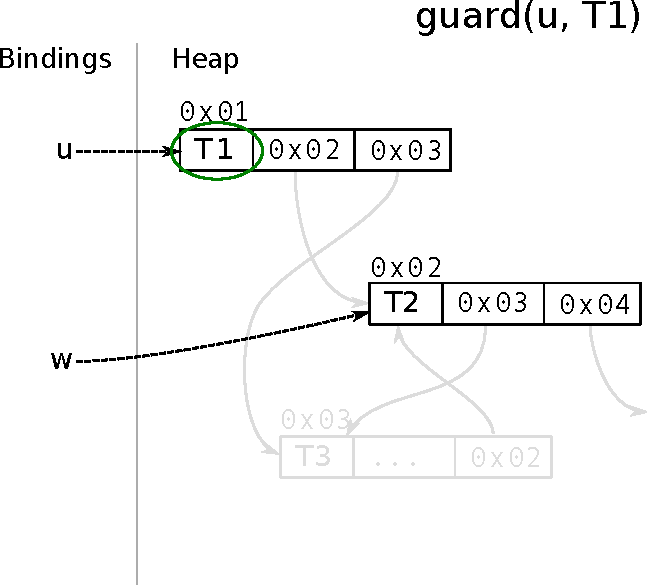
\includegraphics[scale=0.8]{figures/guard02}
\end{frame}

\begin{frame}[plain]
  \frametitle{Operations: Guard}
  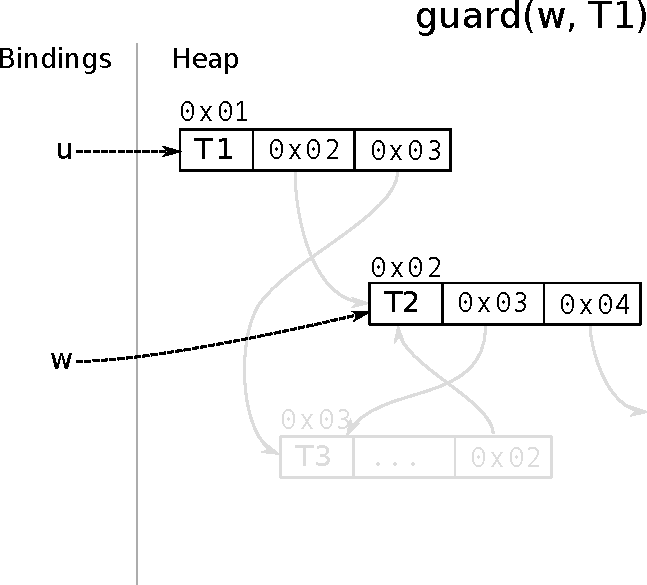
\includegraphics[scale=0.8]{figures/guard03}
\end{frame}

\begin{frame}[plain]
  \frametitle{Operations: Guard}
  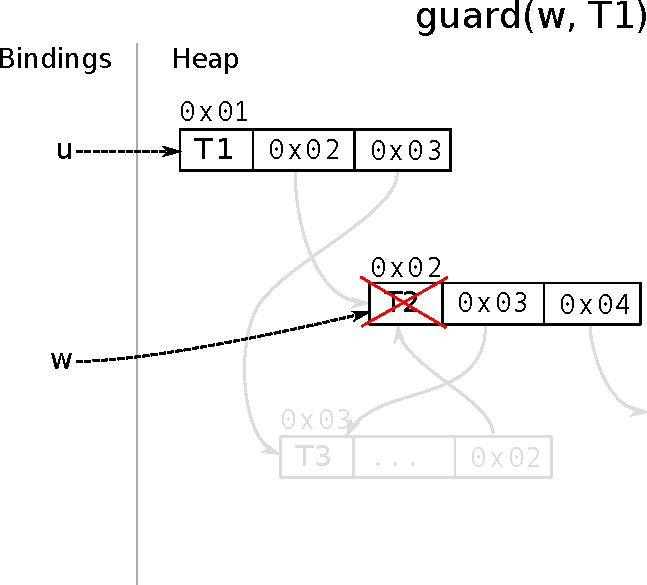
\includegraphics[scale=0.8]{figures/guard04}
\end{frame}

\begin{frame}
  \frametitle{Optimization by Online Partial Evaluation}
  \begin{itemize}
      \item Trace is optimized using online partial evaluation
      \item part of the runtime heap is modelled in the \emph{static heap}
      \item static heap contains objects that are allocated within the trace
      \item (as opposed to before the trace is executed)
      \pause
      \item operations acting on the static heap can be executed
      \item follows operational semantics
      \item all others need to be residualized
      \item all fairly straightforward
  \end{itemize}
\end{frame}


\begin{frame}[plain]
  \frametitle{Optimizing New}
  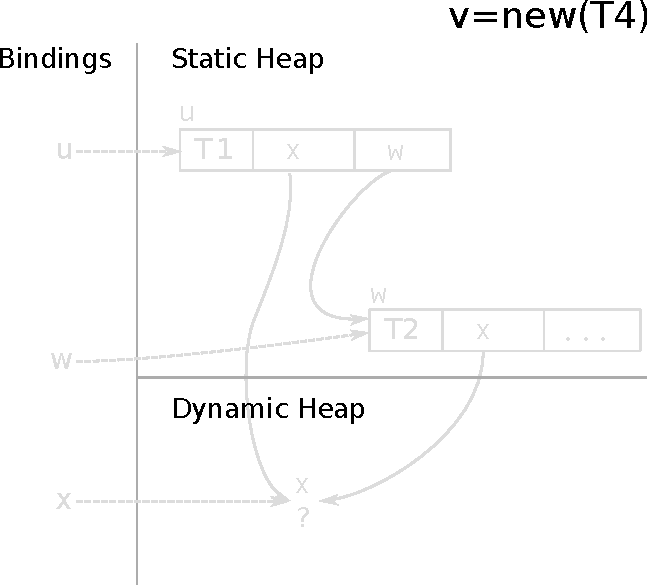
\includegraphics[scale=0.8]{figures/opt_new1}
\end{frame}

\begin{frame}[plain]
  \frametitle{Optimizing New}
  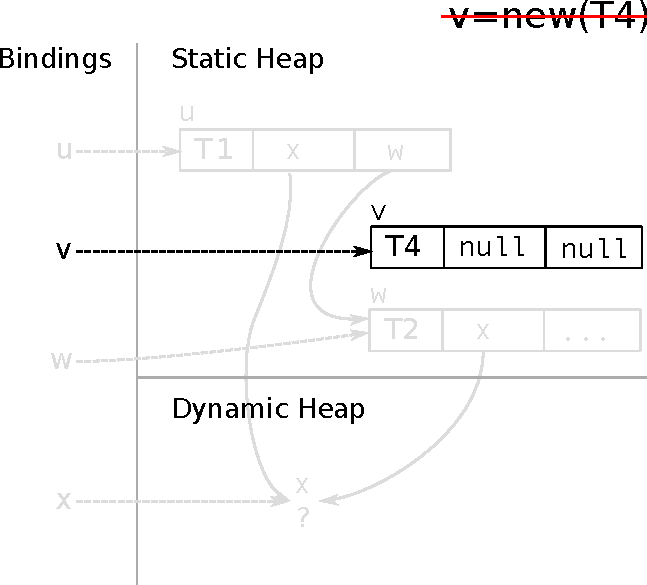
\includegraphics[scale=0.8]{figures/opt_new2}
\end{frame}

\begin{frame}[plain]
  \frametitle{Optimizing Get}
  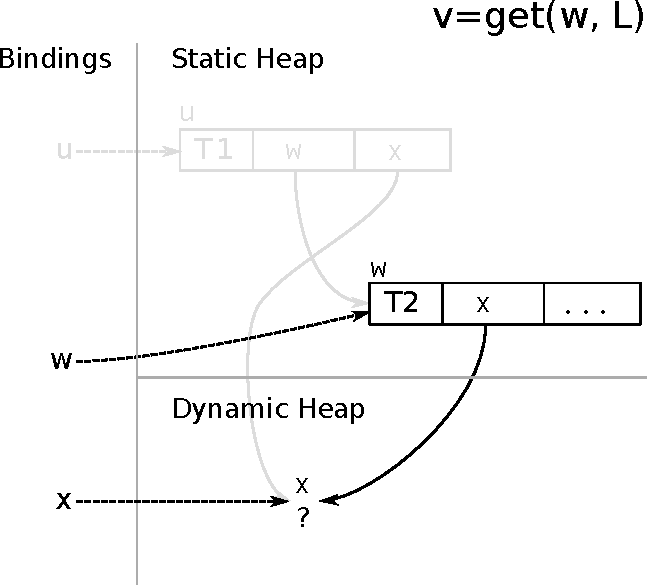
\includegraphics[scale=0.8]{figures/opt_get1}
\end{frame}

\begin{frame}[plain]
  \frametitle{Optimizing Get}
  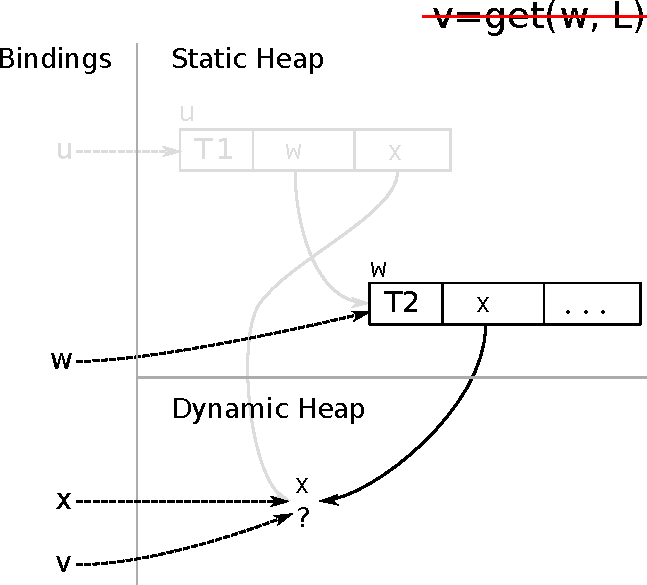
\includegraphics[scale=0.8]{figures/opt_get2}
\end{frame}

\begin{frame}[plain]
  \frametitle{Optimizing Get}
  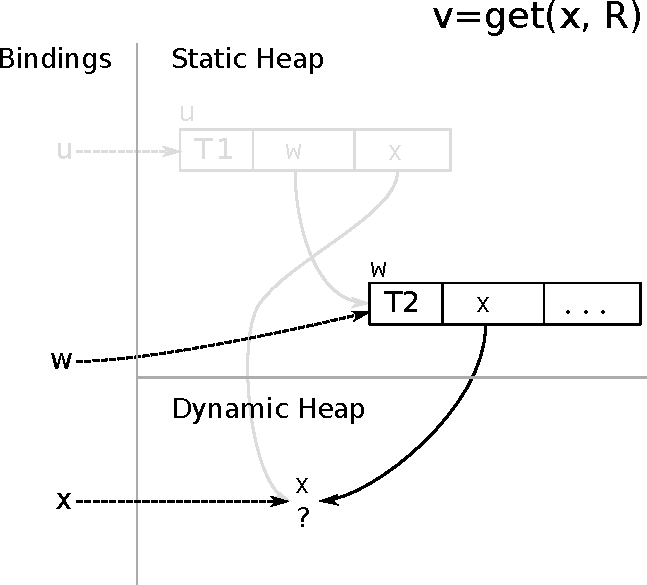
\includegraphics[scale=0.8]{figures/opt_get3}
\end{frame}

\begin{frame}[plain]
  \frametitle{Optimizing Get}
  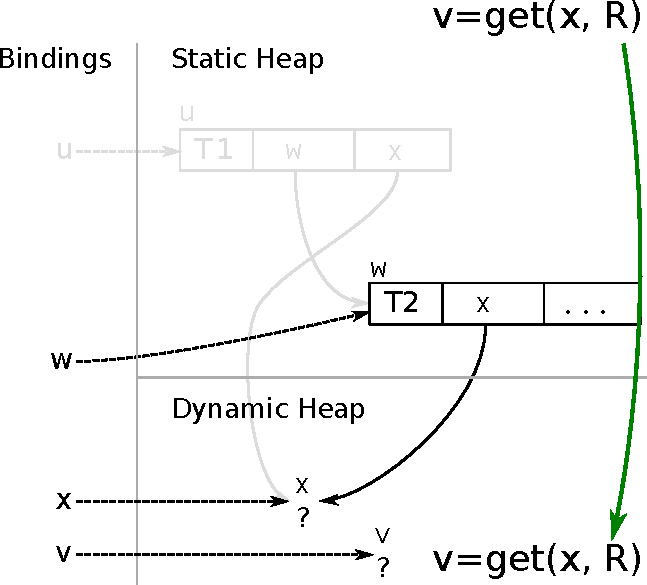
\includegraphics[scale=0.8]{figures/opt_get4}
\end{frame}

\begin{frame}[plain]
  \frametitle{Optimizing Guard}
  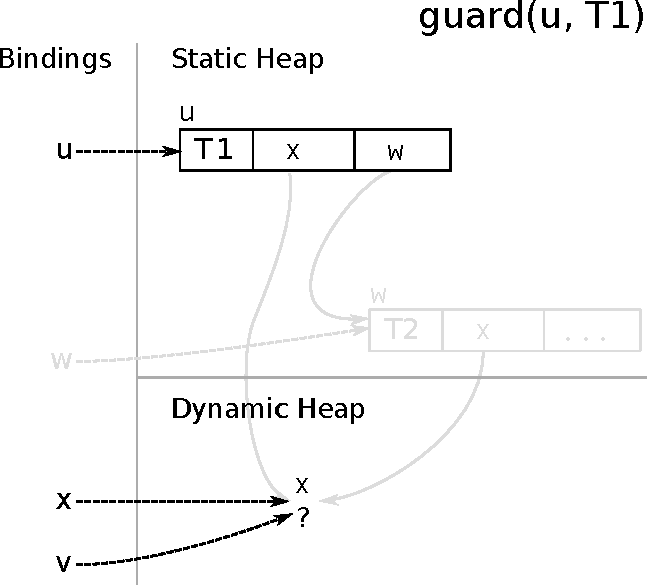
\includegraphics[scale=0.8]{figures/opt_guard1}
\end{frame}

\begin{frame}[plain]
  \frametitle{Optimizing Guard}
  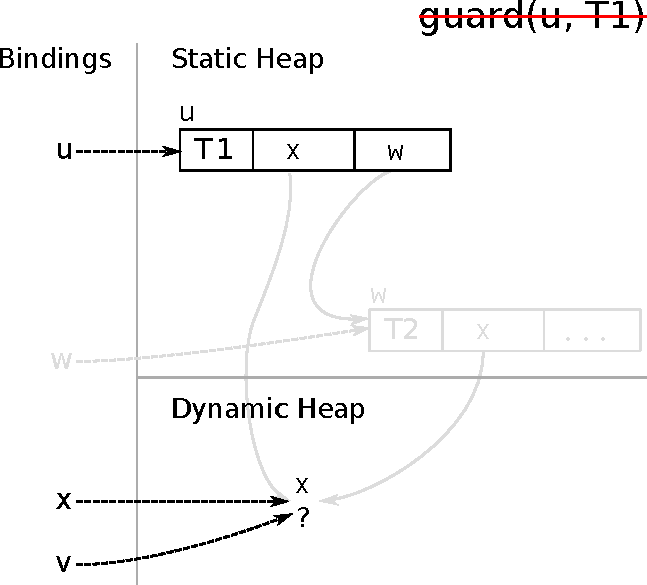
\includegraphics[scale=0.8]{figures/opt_guard2}
\end{frame}

\begin{frame}[plain]
  \frametitle{Optimizing Guard}
  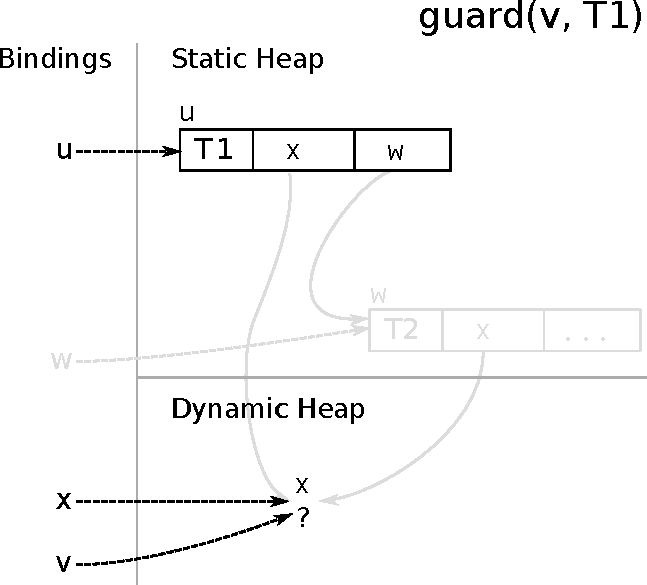
\includegraphics[scale=0.8]{figures/opt_guard3}
\end{frame}

\begin{frame}[plain]
  \frametitle{Optimizing Guard}
  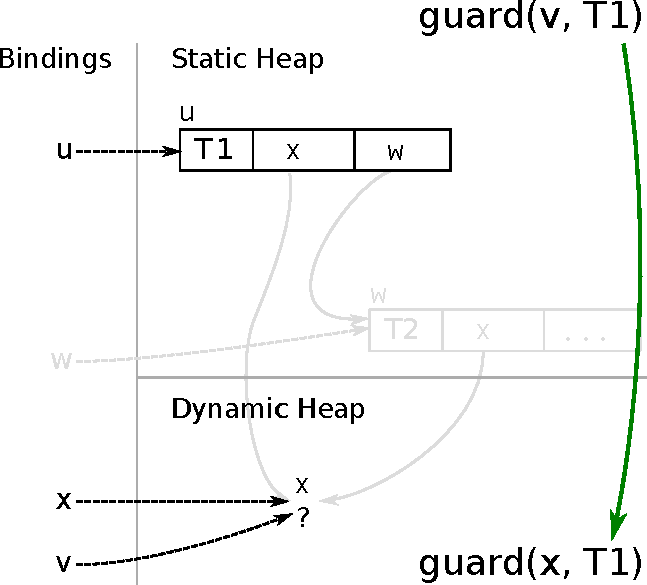
\includegraphics[scale=0.8]{figures/opt_guard4}
\end{frame}

\begin{frame}[plain]
  \frametitle{Optimizing Set}
  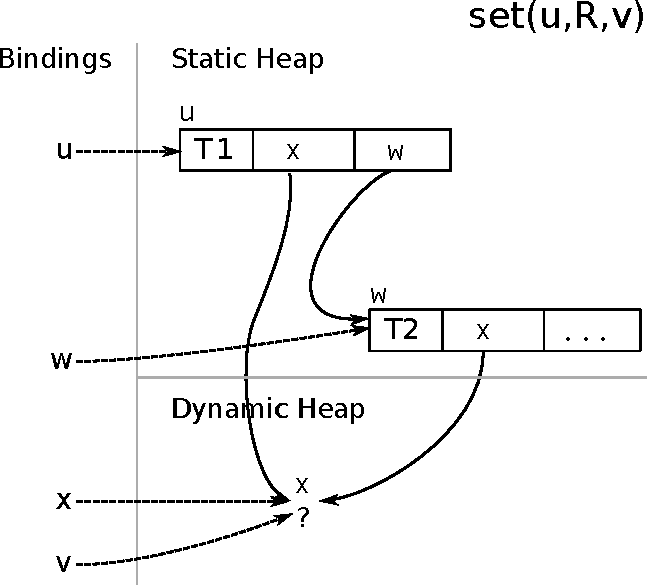
\includegraphics[scale=0.8]{figures/opt_set1}
\end{frame}

\begin{frame}[plain]
  \frametitle{Optimizing Set}
  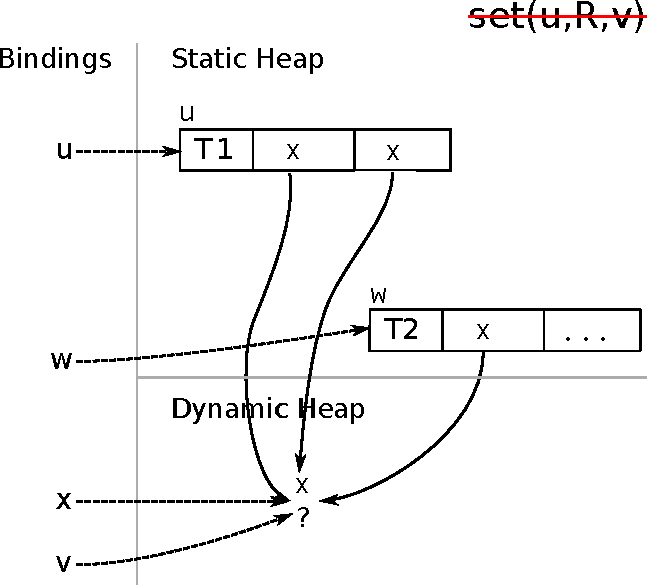
\includegraphics[scale=0.8]{figures/opt_set2}
\end{frame}

\begin{frame}
  \frametitle{Lifting}
  Problem: What happens if we write a static object into a dynamic one?
  \pause
  \begin{itemize}
      \item lose track of the static object because of possibility of aliasing
      \item need to \emph{lift} the static object
      \item lifting produces operations that recreate the static object
      \pause
      \item needs to be careful due to recursive structures
  \end{itemize}
\end{frame}


\begin{frame}[plain]
  \frametitle{Optimizing Set}
  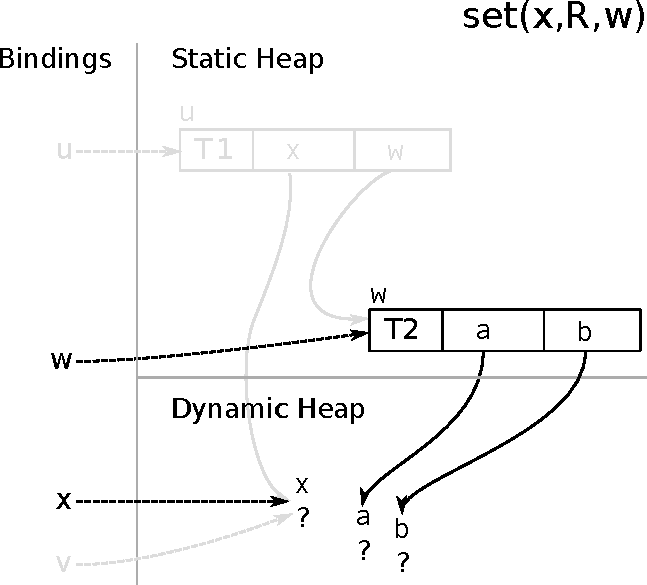
\includegraphics[scale=0.8]{figures/opt_set_dynamic1}
\end{frame}

\begin{frame}[plain]
  \frametitle{Optimizing Set}
  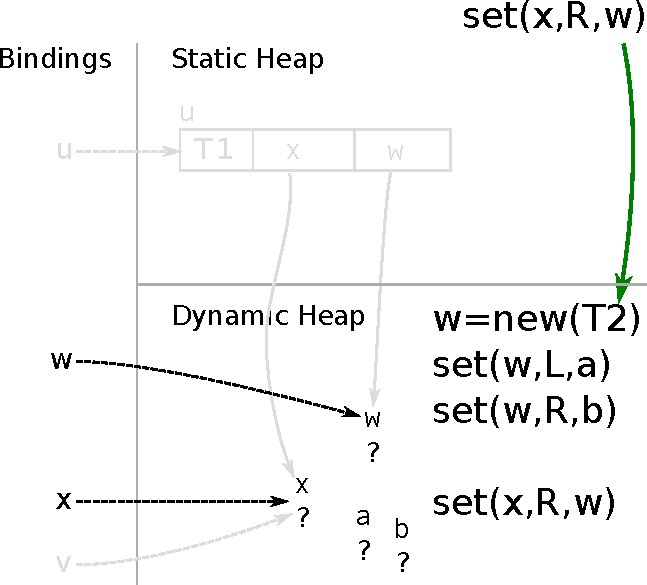
\includegraphics[scale=0.8]{figures/opt_set_dynamic2}
\end{frame}

\begin{frame}
  \frametitle{Properties of the Optimization}
  \begin{itemize}
      \item output trace is never longer than input trace
      \item runtime linear in the length of the trace
  \end{itemize}
  \pause
  \begin{block}{Implementation}
      \begin{itemize}
          \item about 400 lines of code
          \item some added complexity over presentation
          \item objects with arbitrary numbers of fields
          \item array support
      \end{itemize}
  \end{block}
\end{frame}


\begin{frame}[plain]
    \frametitle{Optimizing the Example Trace}
\only<1>
{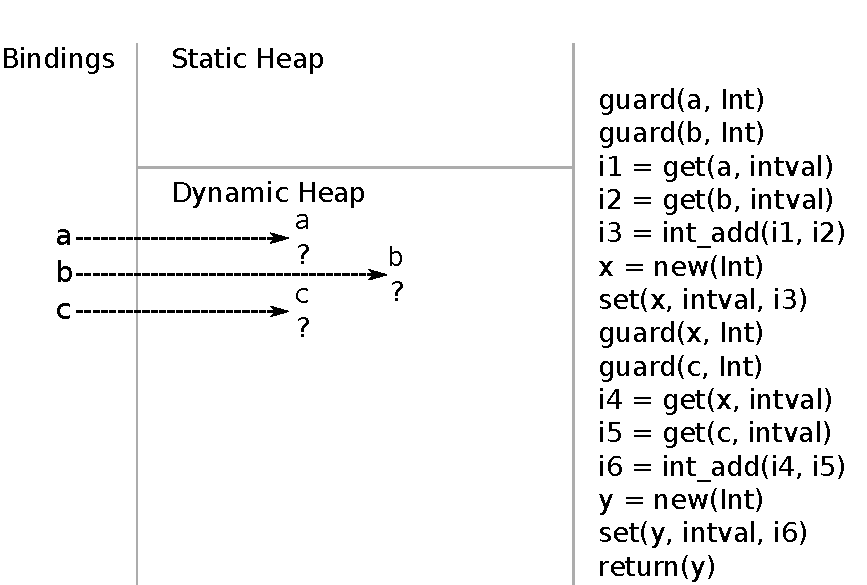
\includegraphics[scale=0.8]{figures/ex00}}
\only<2>
{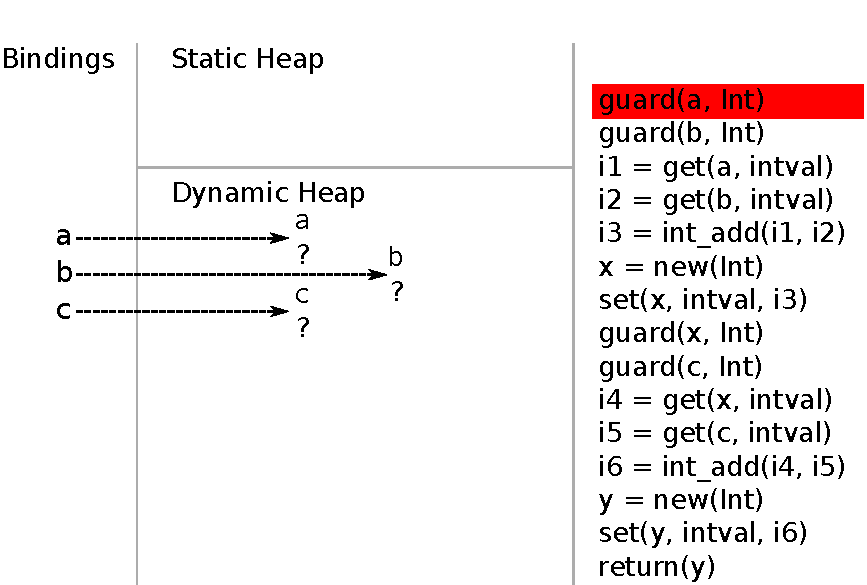
\includegraphics[scale=0.8]{figures/ex01}}
\only<3>
{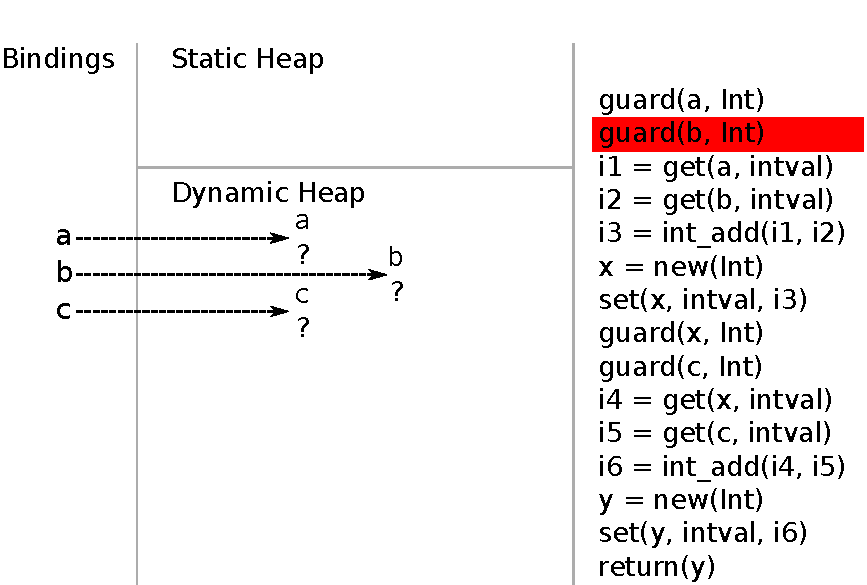
\includegraphics[scale=0.8]{figures/ex02}}
\only<4>
{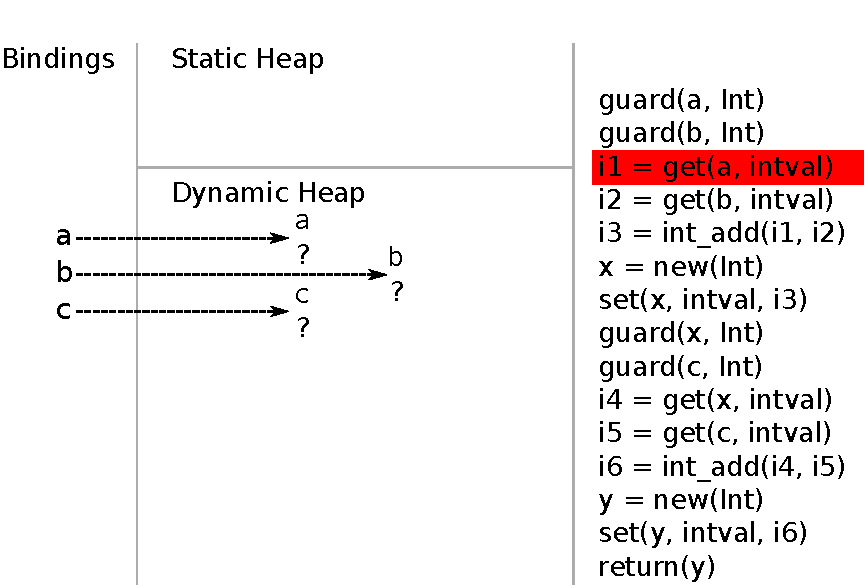
\includegraphics[scale=0.8]{figures/ex03}}
\only<5>
{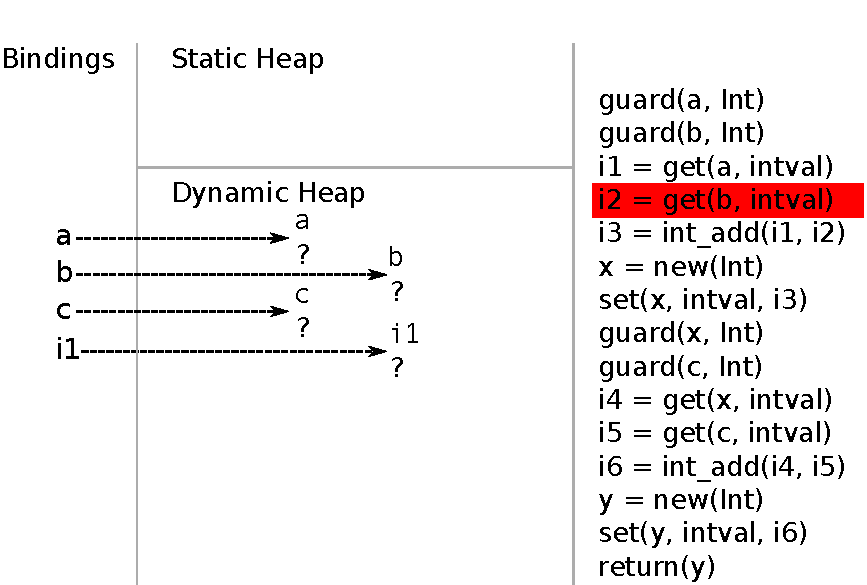
\includegraphics[scale=0.8]{figures/ex04}}
\only<6>
{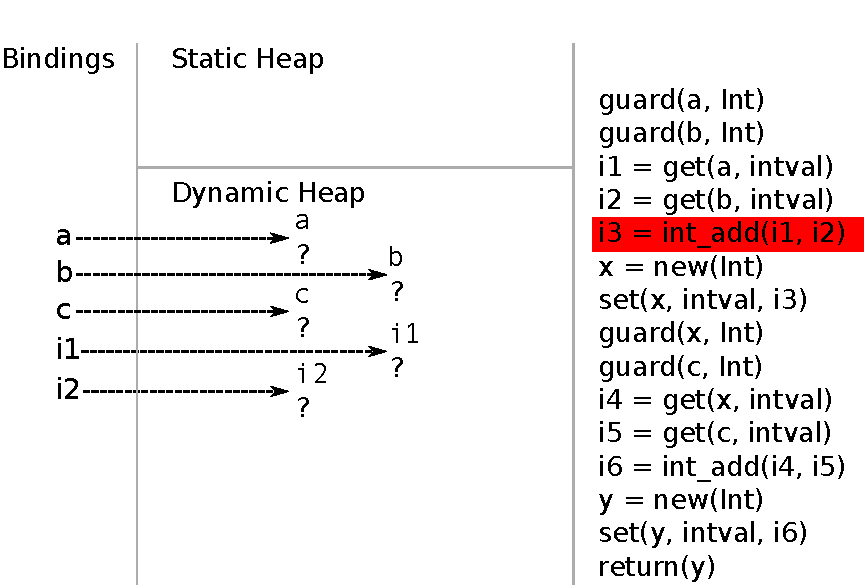
\includegraphics[scale=0.8]{figures/ex05}}
\only<7>
{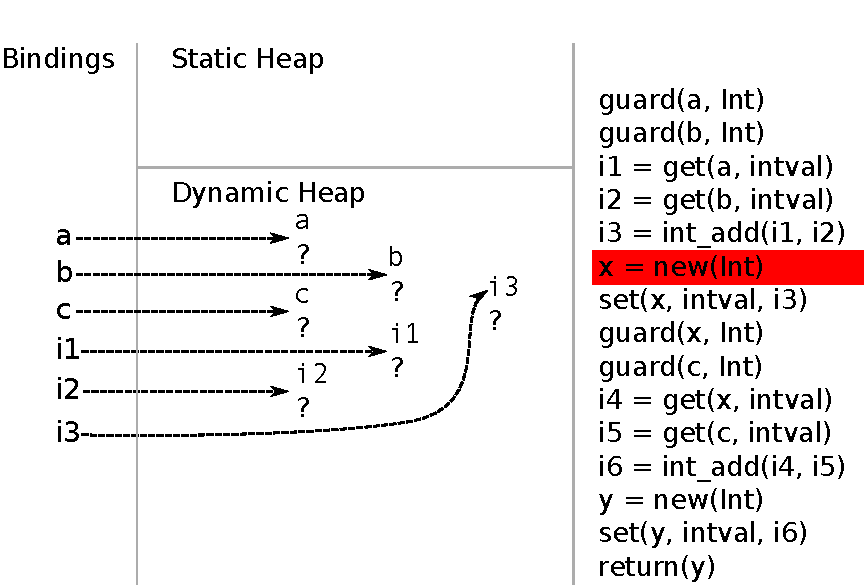
\includegraphics[scale=0.8]{figures/ex06}}
\only<8>
{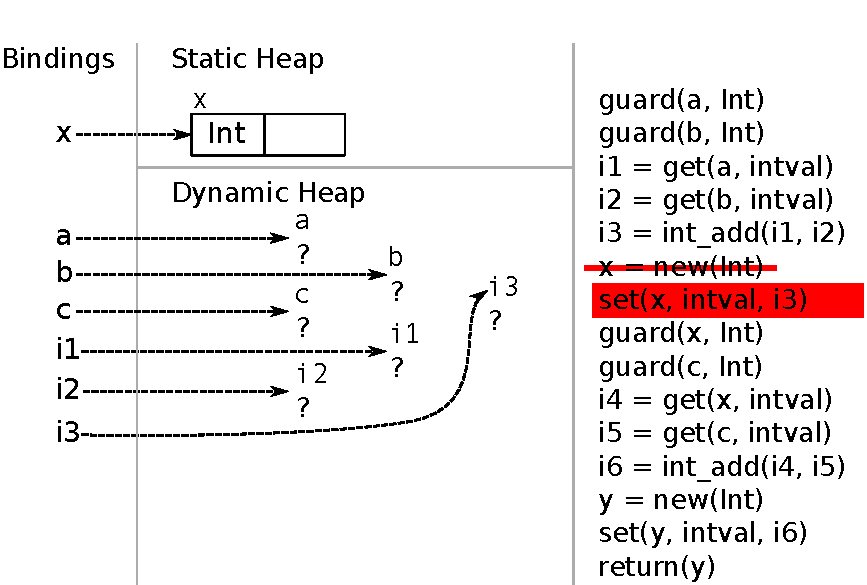
\includegraphics[scale=0.8]{figures/ex07}}
\only<9>
{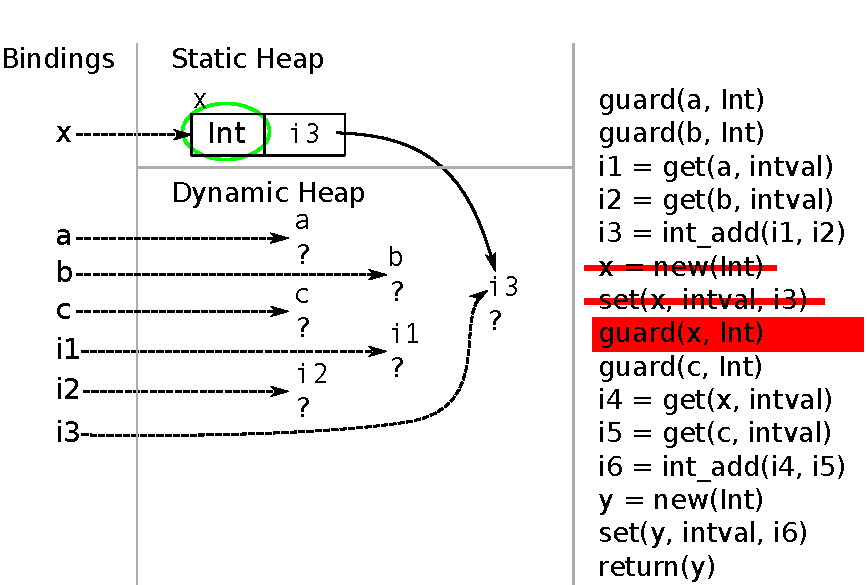
\includegraphics[scale=0.8]{figures/ex08}}
\only<10>
{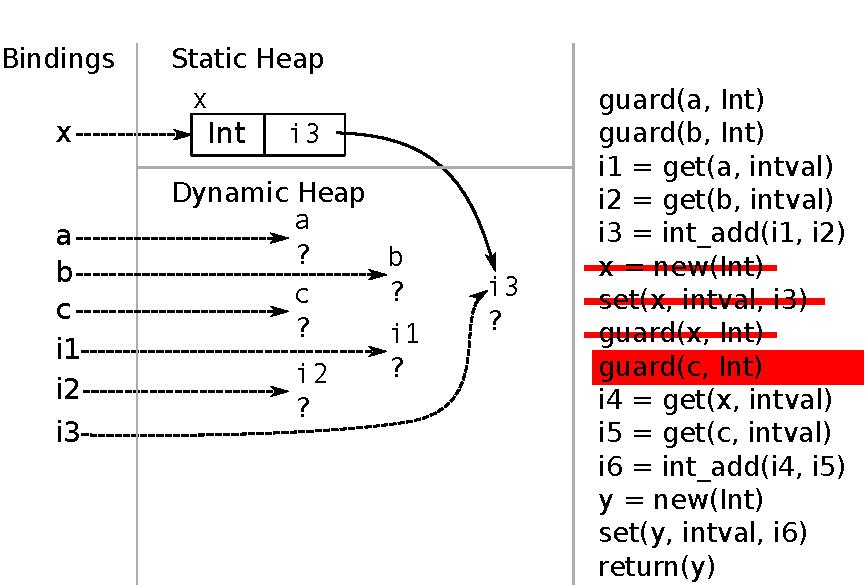
\includegraphics[scale=0.8]{figures/ex09}}
\only<11>
{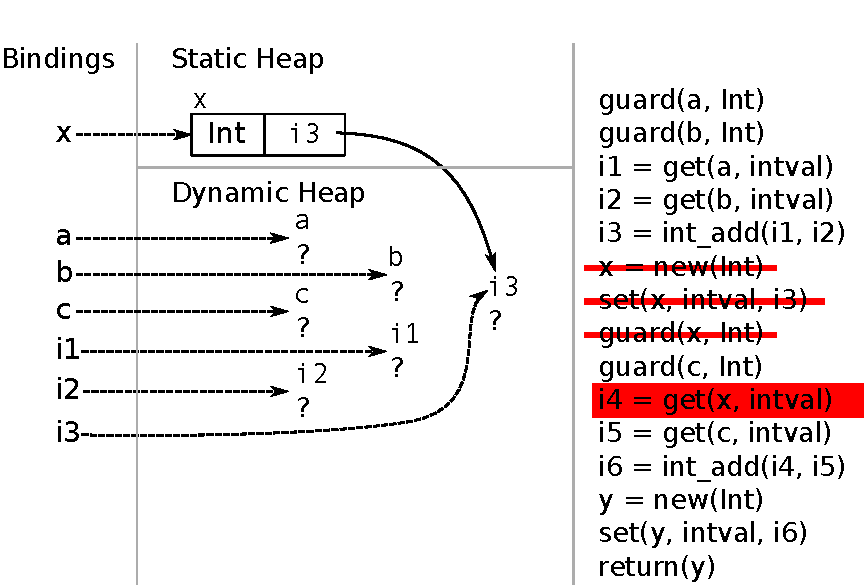
\includegraphics[scale=0.8]{figures/ex10}}
\only<12>
{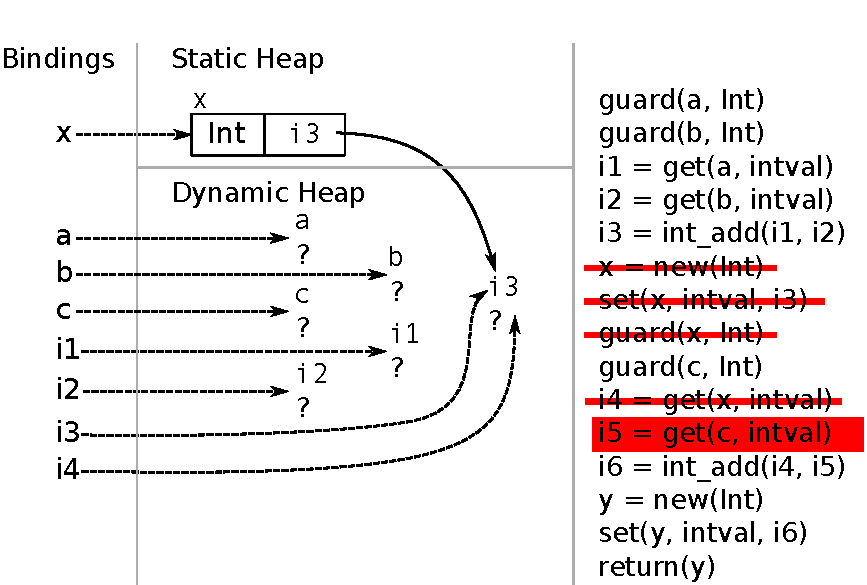
\includegraphics[scale=0.8]{figures/ex11}}
\only<13>
{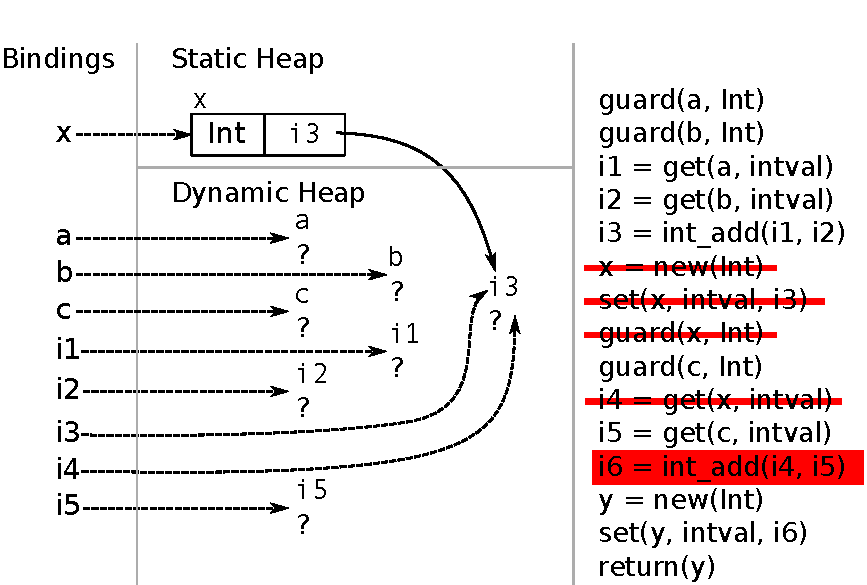
\includegraphics[scale=0.8]{figures/ex12}}
\only<14>
{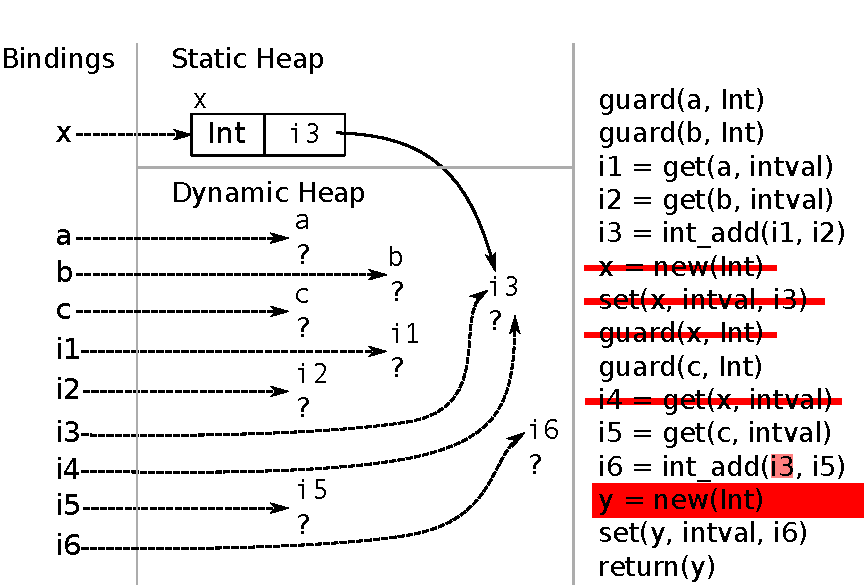
\includegraphics[scale=0.8]{figures/ex13}}
\only<15>
{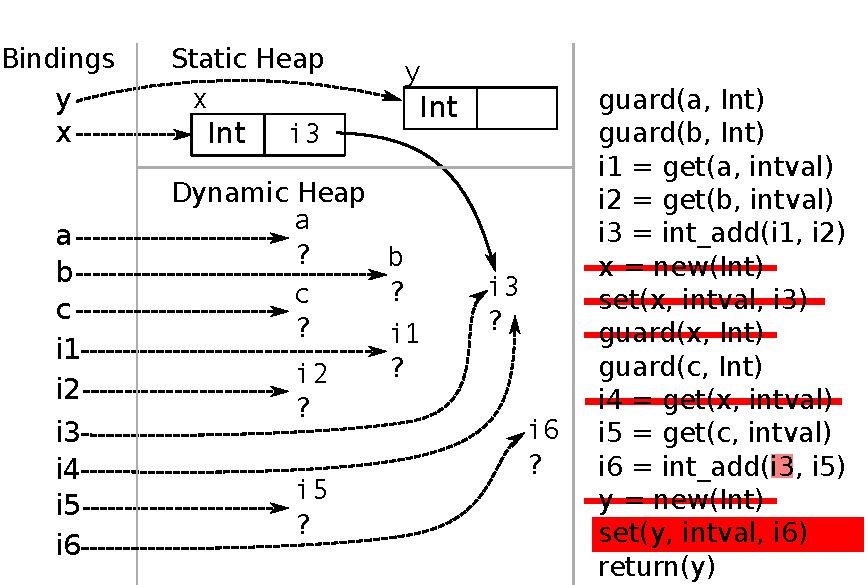
\includegraphics[scale=0.8]{figures/ex14}}
\only<16>
{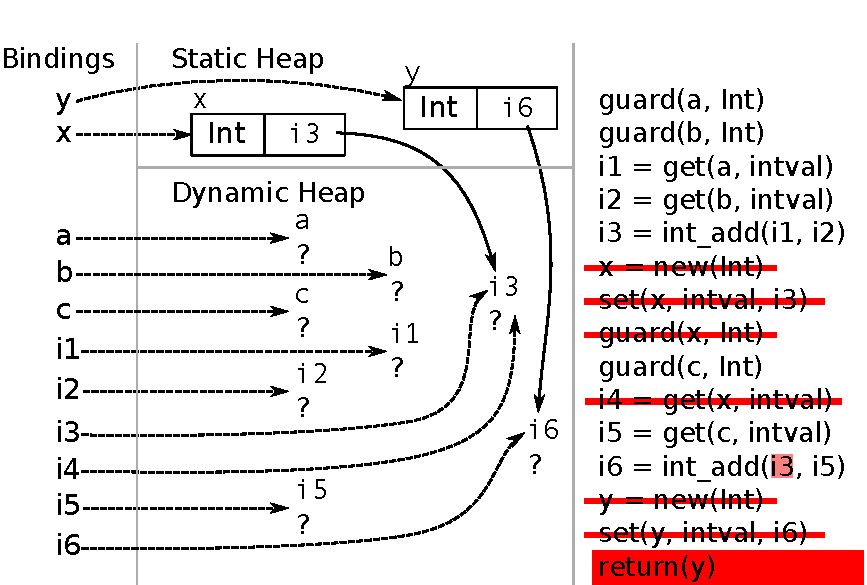
\includegraphics[scale=0.8]{figures/ex15}}
\only<17>
{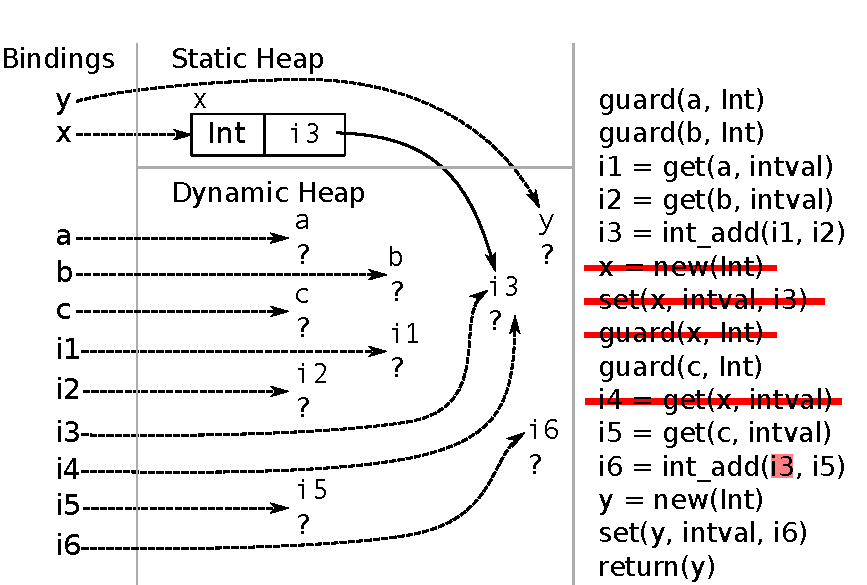
\includegraphics[scale=0.8]{figures/ex16}}
\end{frame}

\section{Benchmarks}

\begin{frame}
  \frametitle{Benchmark Results}
  \begin{itemize}
      \item to evaluate the optimization we used PyPy's Python interpreter with real-world programs
      \begin{itemize}
          \item interpreter is about 30'000 lines of code
      \end{itemize}
      \pause
      \item optimization can remove
      \begin{itemize}
          \item 70\% of all \texttt{new} operations
          \item 14\% of all \texttt{get/set} operations
          \item 93\% of all \texttt{guard} operations
      \end{itemize}
      \pause
      \item Timings improve by a factor between 1.1 and 6.95
      \item outperforming standard Python on all benchmarks but two
  \end{itemize}
\end{frame}

\begin{frame}
  \frametitle{Benchmark}
  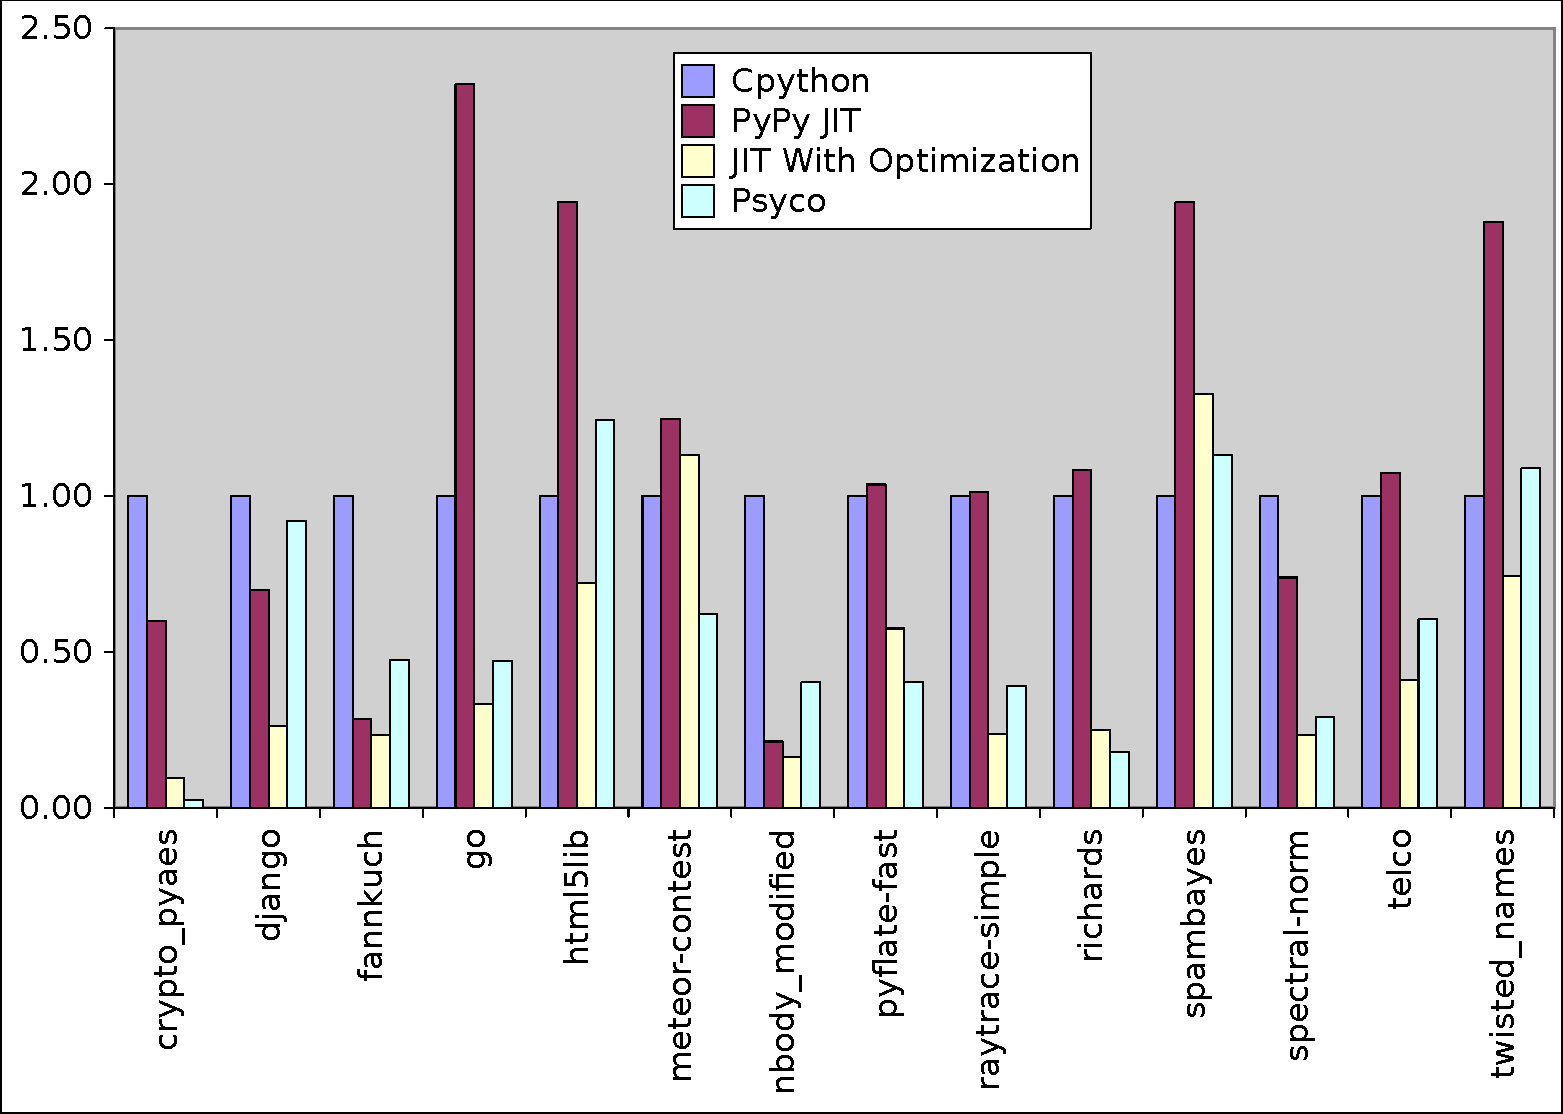
\includegraphics[scale=0.4]{figures/benchmarks}
\end{frame}

\begin{frame}
  \frametitle{Conclusion}
  \begin{itemize}
      \item We propose a very simple partial-evaluation-based optimization for tracing
      JITs of dynamic languages that:
      \begin{itemize}
          \item can remove a lot of allocations and type checks in practical
          programs. 
          \item is efficient and effective.
          \item has no control issues because all control decisions are made by
          the tracing JIT.
      \end{itemize}
      \pause
      \item We claim that this is a general strategy to get rid of control
      problems by simply observing the runtime behaviour of the program.
  \end{itemize}
\end{frame}


\begin{frame}
  \frametitle{Backup Slides}
\end{frame}

\begin{frame}
  \frametitle{What About Correctness?}
  \begin{itemize}
      \item We haven't proven correctness yet
      \item should not be too hard
      \item lifting needs to be carefully handled
  \end{itemize}
\end{frame}

\begin{frame}
  \frametitle{Comparison to Escape Analysis}
  \begin{itemize}
      \item Effect very similar to escape analysis
      \item Escape analysis needs a complex upfront analysis
      \item our optimization automatically has a lot of context, due to the inlining tracing does
      \item our optimization can optimize operations on objects even if they escape later
  \end{itemize}
\end{frame}

\begin{frame}[containsverbatim]
  \frametitle{Comparison to "Dynamic Typing"/Boxing Analysis}
  \begin{itemize}
      \item those optimizations work ahead of time
      \item don't work for many dynamic languages, where the source simply does not contain enough information
  \end{itemize}
  \begin{block}{Python Example:}
  \begin{verbatim}
def sum(container, initial):
    result = initial
    for element in container:
        result = result + element
    return result
  \end{verbatim}
  \end{block}
\end{frame}

\end{document}
